\documentclass[11pt,a4paper]{article}
\usepackage[italian]{babel}
\usepackage{fontspec}
\setmainfont{texgyrepagella}[Extension=.otf,UprightFont=*-regular,BoldFont=*-bold,ItalicFont=*-italic,BoldItalicFont=*-bolditalic]
\setmonofont{Menlo}[Scale=0.85]
\usepackage[margin=2.2cm]{geometry}
\usepackage{graphicx,booktabs,amsmath,amssymb,enumitem,xcolor}
\usepackage[most]{tcolorbox}
\usepackage[hidelinks]{hyperref}
\usepackage{titlesec}
\usepackage{float}
\usepackage{fancyvrb}

\definecolor{idea}{HTML}{1F6FB2}
\definecolor{attn}{HTML}{C0392B}
\definecolor{exam}{HTML}{27AE60}

\newtcolorbox{idea}{colback=idea!6,colframe=idea,boxrule=0.6pt,arc=2pt,left=6pt,right=6pt,top=4pt,bottom=4pt,
  fonttitle=\bfseries\small,title=L'idea in breve}
\newtcolorbox{attenzione}{colback=attn!5,colframe=attn,boxrule=0.6pt,arc=2pt,left=6pt,right=6pt,top=4pt,bottom=4pt,
  fonttitle=\bfseries\small,title=Attenzione: il notebook sbaglia o confonde}
\newtcolorbox{esame}{colback=exam!6,colframe=exam,boxrule=0.6pt,arc=2pt,left=6pt,right=6pt,top=4pt,bottom=4pt,
  fonttitle=\bfseries\small,title=Da ricordare per l'esame}
\newtcolorbox{soluzione}{colback=black!3,colframe=black!45,boxrule=0.6pt,arc=2pt,left=6pt,right=6pt,top=4pt,bottom=4pt,
  fonttitle=\bfseries\small,title=Soluzione (eseguita)}

\titleformat{\section}{\Large\bfseries\color{idea}}{\thesection}{0.6em}{}
\titleformat{\subsection}{\large\bfseries}{\thesubsection}{0.6em}{}
\setlist{itemsep=2pt,topsep=3pt}
\setlength{\parindent}{0pt}
\setlength{\parskip}{5pt}
\newcommand{\code}[1]{\texttt{#1}}
\fvset{fontsize=\small}
\setlength{\emergencystretch}{3em}

\begin{document}

\begin{center}
{\LARGE\bfseries Computer Vision, Lezione 7}\\[3pt]
{\large Laboratorio: Fourier sulle immagini e classificazione con banchi di filtri}\\[3pt]
{\small Appunti ricavati dai notebook in \code{Lessons/L7/lab/} (\code{demo}, \code{filter\_bank}, \code{06-image-blending})}
\end{center}

\section*{Come leggere questi appunti}

La lezione 4 faceva spettro e convoluzione su segnali 1D (audio). Questo laboratorio fa \textbf{la stessa cosa in 2D, sulle immagini}, e poi usa le convoluzioni come estrattori di feature per un classificatore.

\begin{center}
\begin{tabular}{@{}lll@{}}
\toprule
Parte & Notebook & Domanda a cui risponde \\
\midrule
1 & \code{demo.ipynb} & Com'è fatto lo spettro di un'immagine e come si filtra? \\
2 & \code{filter\_bank.ipynb} & Quanto si classifica bene con filtri fissi scelti a mano? \\
3 & \code{06-image-blending} & Identico a quello della lezione 6: vedi sezione 3. \\
\bottomrule
\end{tabular}
\end{center}

Teoria collegata: convoluzione e teorema di convoluzione (lezione 3), piramidi e aliasing (lezione 6), FFT 1D (laboratorio 4).

Riquadri: \textcolor{idea}{\textbf{blu}} = il concetto in due righe, \textcolor{attn}{\textbf{rosso}} = punti in cui il notebook sbaglia o confonde, \textcolor{exam}{\textbf{verde}} = cosa ricordare, \textbf{grigio} = soluzione di un esercizio, eseguita.

\medskip
\textbf{Tre parole da sapere prima di iniziare}
\begin{itemize}
  \item \textbf{Frequenza spaziale}: quante volte un motivo si ripete per pixel, in \emph{cicli/pixel}. Va da $-0.5$ a $0.5$ (Nyquist). Una frequenza 2D è una coppia $(f_x, f_y)$.
  \item \textbf{Spettro 2D}: la FFT dell'immagine (\code{np.fft.fft2}). Si disegna il modulo in scala log, con la frequenza zero al centro (\code{fftshift}).
  \item \textbf{Banco di filtri}: una lista di kernel. Ogni kernel convoluto con l'immagine dà una mappa di risposta; le mappe, ridotte, diventano le feature del classificatore.
\end{itemize}

\newpage
%=====================================================================
\section{Fourier e convoluzione sulle immagini (\code{demo.ipynb})}

Immagine di lavoro: \code{camera} di scikit-image, ritagliata a $256 \times 256$ (\code{[96:352, 128:384]}).

\subsection{Coordinate di Fourier: i fatti da sapere}

\begin{center}
\begin{tabular}{@{}p{6.3cm}p{8.2cm}@{}}
\toprule
Cosa & Come / quanto vale (rieseguito) \\
\midrule
\code{np.fft.fft2(img)} & FFT sulle due assi, uscita $H \times W$ complessa \\
\code{np.fft.fftfreq(W)} & frequenze in cicli/pixel, \emph{nell'ordine della FFT}: $0, 1/W, \dots, $ poi le negative \\
\code{F[0,0] / (H*W)} & media dell'immagine (componente continua, DC): 0.3984 \\
Parseval: $\sum |f|^2 = \sum |F|^2 / (HW)$ & 16143.14 = 16143.14 \\
\code{ifft2(fft2(img)).real} & ritorna l'immagine, errore massimo $5.6\cdot 10^{-16}$ \\
\code{fftshift} / \code{ifftshift} & porta DC al centro per disegnare; \code{ifftshift} prima di invertire uno spettro centrato \\
\bottomrule
\end{tabular}
\end{center}

\begin{figure}[H]\centering
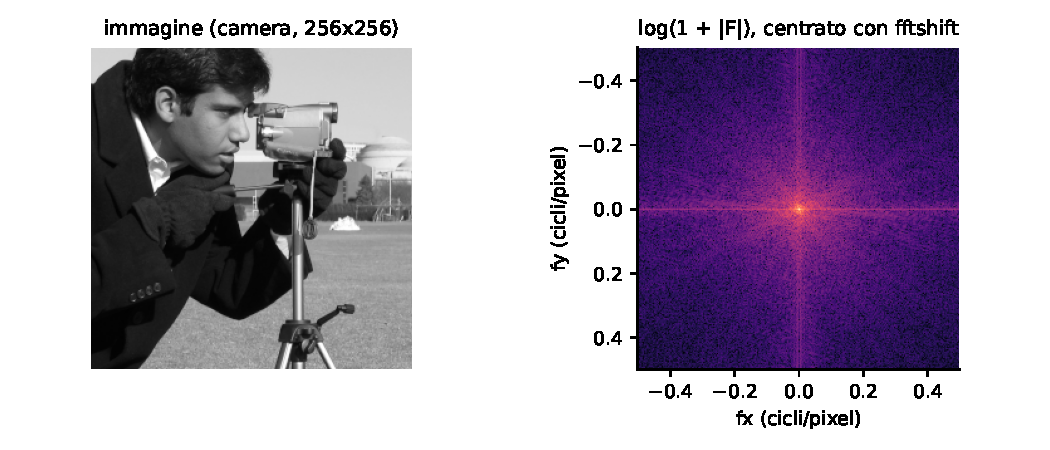
\includegraphics[width=0.75\linewidth]{fig/spectrum.pdf}
\caption{Lo spettro di un'immagine naturale: quasi tutta l'energia vicino al centro (basse frequenze). La croce orizzontale e verticale viene dai bordi dell'immagine: la FFT la tratta come periodica e il salto tra lato destro e sinistro è un bordo netto.}
\end{figure}

\subsection{Onde semplici: prevedere lo spettro}

Un'onda $g[y,x] = \cos\big(2\pi(k_x x/W + k_y y/H)\big)$ con $k_x, k_y$ interi ha \textbf{due picchi} in $\pm(k_y, k_x)$, ognuno di modulo $HW/2$ (qui 32768, verificato).

\begin{figure}[H]\centering
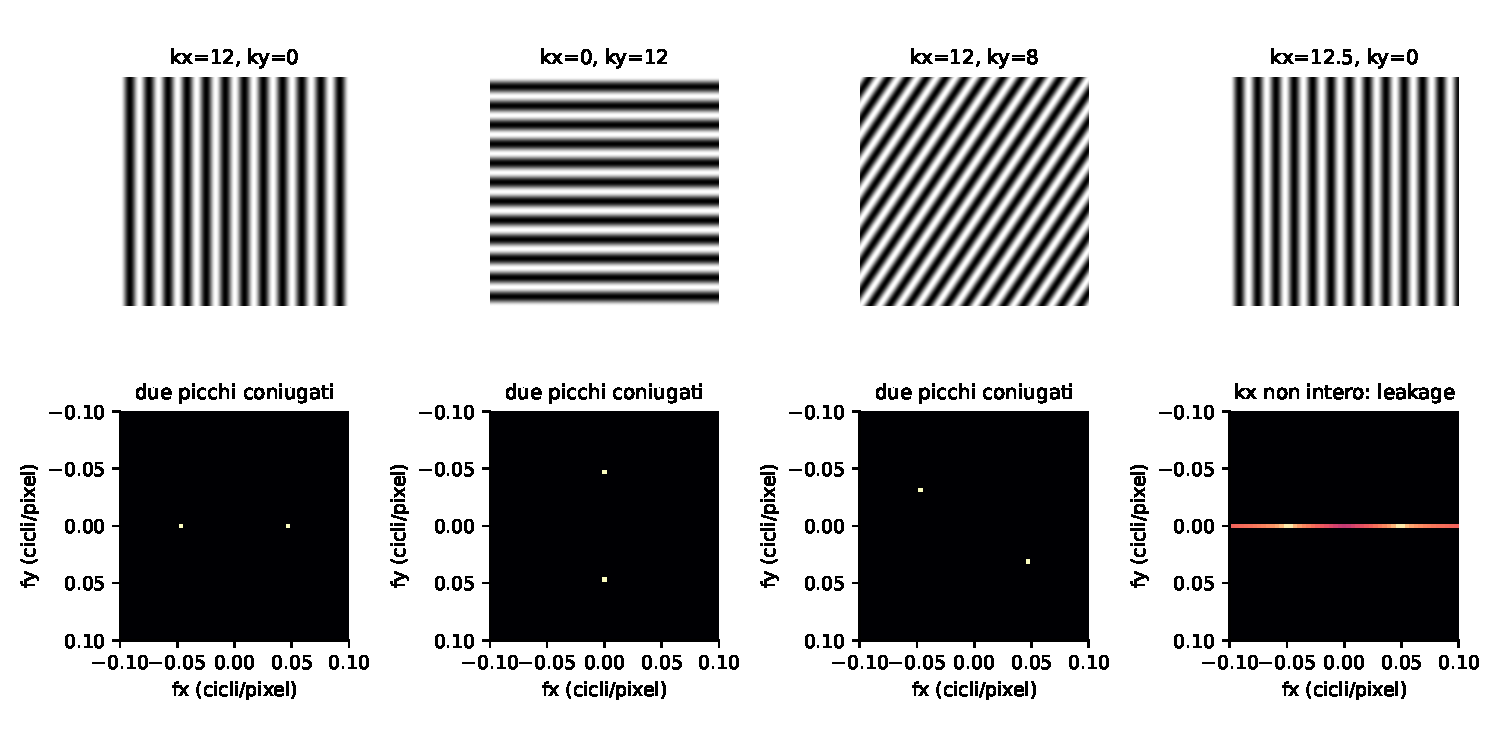
\includegraphics[width=\linewidth]{fig/gratings.pdf}
\caption{Zoom sulla zona $|f| < 0.1$. Le strisce verticali ($k_x = 12$) danno picchi sull'asse orizzontale: il vettore $(k_x/W, k_y/H)$ è \emph{perpendicolare} alle strisce. A destra $k_x = 12.5$ non è intero: l'onda non si chiude sul bordo e l'energia si spande su tutta la riga (spectral leakage): 256 bin sopra l'1\% del massimo, contro 2.}
\end{figure}

Risposte agli esercizi semplici della cella 5:
\begin{itemize}
  \item Cambiando $(k_x, k_y)$: la \textbf{direzione} dei picchi è perpendicolare alle strisce, la \textbf{distanza} dal centro è la frequenza (strisce più fitte = picchi più lontani).
  \item Frequenza non intera: leakage, come in figura.
  \item Somma di onde: lo spettro è la somma degli spettri (la FFT è lineare), quindi una coppia di picchi per ogni onda.
\end{itemize}

\subsection{Modulo, fase e traslazione}

Spostare l'immagine \textbf{cambia solo la fase} dello spettro, non il modulo:
\[
\text{shift di } (d_y, d_x) \;\Longleftrightarrow\; F \cdot e^{-2\pi i (f_y d_y + f_x d_x)}
\]
Il notebook lo prova con \code{np.roll(image, (27, -19))}: la ricostruzione con la rampa di fase coincide con l'immagine spostata e il modulo della FFT non cambia (entrambe le asserzioni passano). Vale per lo spostamento \emph{circolare} (\code{np.roll}): quello che esce da un lato rientra dall'altro.

\begin{idea}
Il modulo dice \emph{quali} frequenze ci sono, la fase dice \emph{dove} stanno. Uno spostamento non cambia il contenuto in frequenza, quindi non tocca il modulo.
\end{idea}

\subsection{Bordi: cosa c'è fuori dall'immagine}

\code{scipy.signal.convolve2d(img, k, mode="same", boundary=...)}. Il parametro \code{mode} decide solo la \emph{dimensione} dell'uscita; \code{boundary} decide come si estende l'immagine.

\begin{figure}[H]\centering
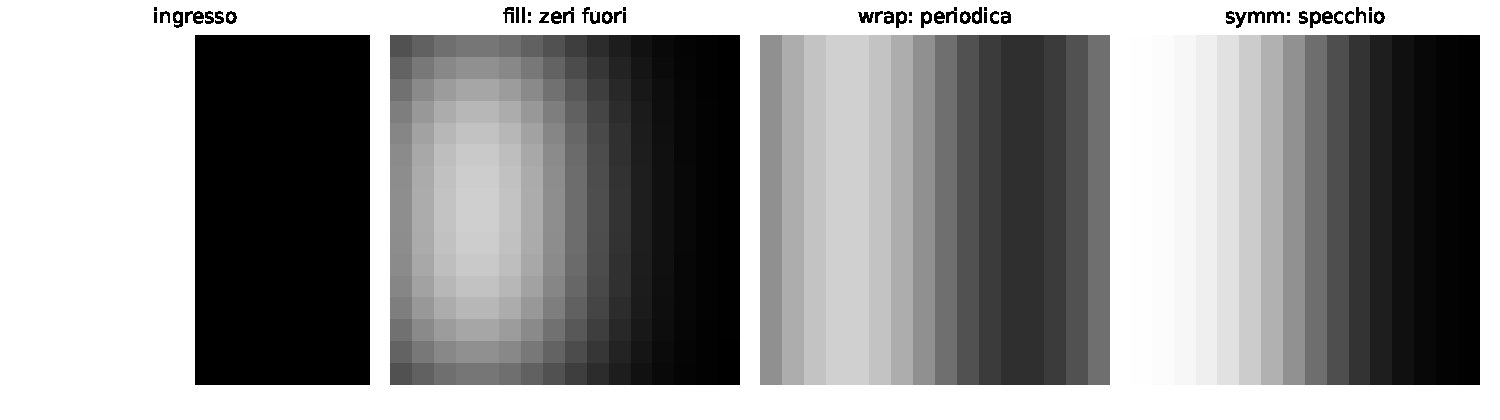
\includegraphics[width=\linewidth]{fig/boundary.pdf}
\caption{Quadrato $16 \times 16$ metà bianco, sfocato con una gaussiana $\sigma = 3$.}
\end{figure}

\begin{center}
\begin{tabular}{@{}lp{6.2cm}cc@{}}
\toprule
\code{boundary} & Estensione & angolo bianco (0,0) & bordo nero (8,15) \\
\midrule
\code{fill} & zeri fuori: i bordi si scuriscono & 0.318 & 0.005 \\
\code{wrap} & periodica: il lato destro (nero) entra a sinistra & 0.563 & 0.437 \\
\code{symm} & specchio, ripetendo il pixel di bordo & 0.993 & 0.007 \\
\bottomrule
\end{tabular}
\end{center}

Verificato: \code{symm} equivale a \code{np.pad(..., mode="symmetric")}, cioè $[1,2,3] \to [\dots 2,1,\,1,2,3,\,3,2 \dots]$ (il pixel di bordo è ripetuto; \code{"reflect"} invece non lo ripete).

\textbf{Collegamento importante}: filtrare moltiplicando nello spettro (\code{fft2}, maschera, \code{ifft2}) equivale a una convoluzione con \code{boundary="wrap"}, perché la DFT tratta l'immagine come periodica.

\subsection{Passa-basso ideale e gaussiano}

Le due maschere del notebook, con $r = \sqrt{f_x^2 + f_y^2}$:
\begin{itemize}
  \item \textbf{ideale}: $M = 1$ se $r \le 0.08$, altrimenti 0 (tiene il 2.0\% dei coefficienti);
  \item \textbf{gaussiana}: $M = \exp(-2\pi^2\sigma^2 r^2)$ con $\sigma = 2$. È la trasformata di un kernel gaussiano spaziale di deviazione standard $\sigma$: verificato, il kernel che corrisponde alla maschera ha std 2.000 pixel.
\end{itemize}

\begin{figure}[H]\centering
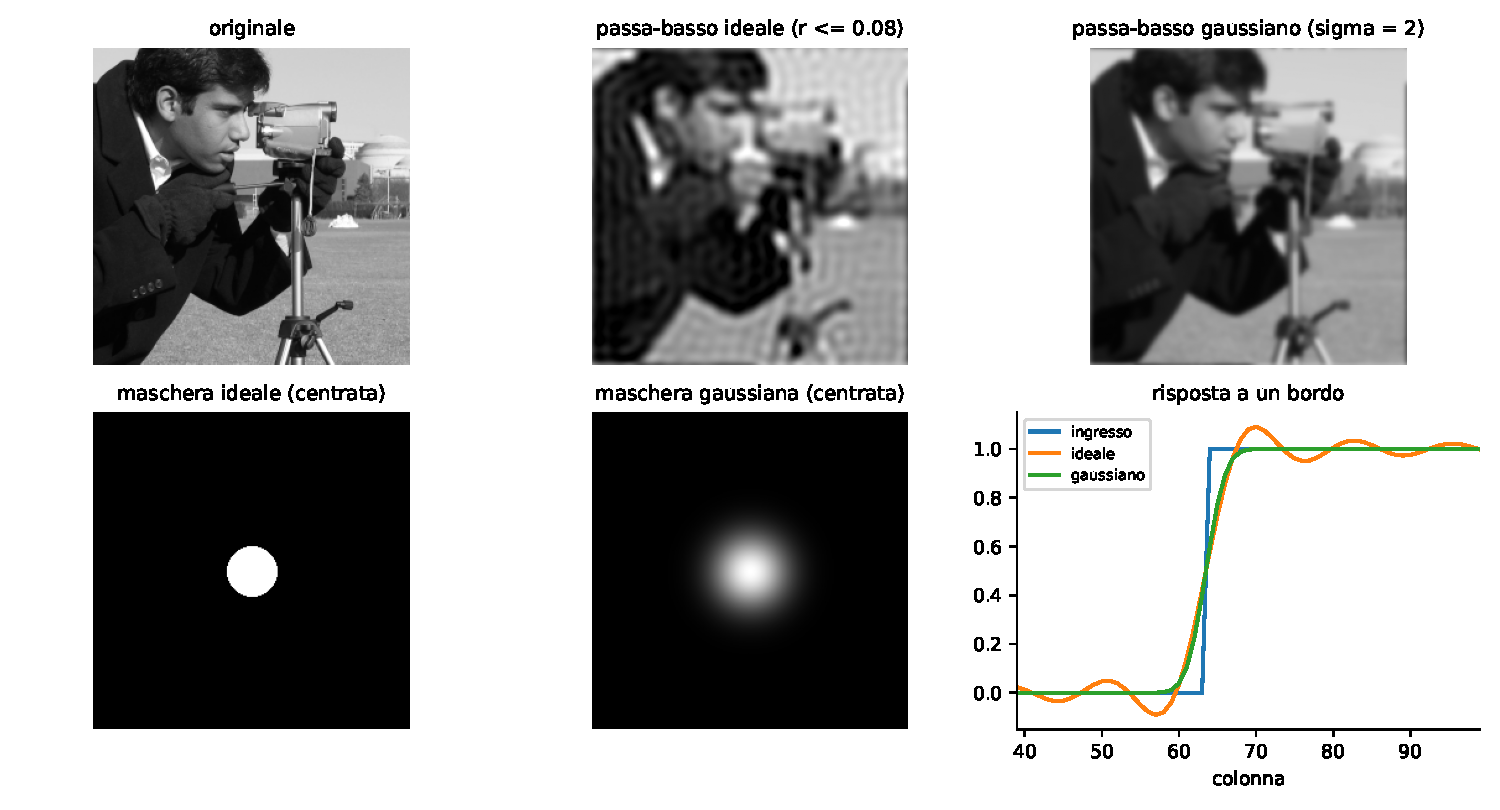
\includegraphics[width=\linewidth]{fig/lowpass.pdf}
\caption{Il passa-basso ideale produce aloni attorno ai contorni (ringing). Sul bordo netto (in basso a destra): l'ideale oscilla tra $-0.091$ e $1.091$ (9\% oltre i valori reali), il gaussiano resta in $[0, 1]$.}
\end{figure}

\begin{idea}
Taglio netto in frequenza = sinc nello spazio = oscillazioni (ringing). La gaussiana non ha taglio netto: nello spazio è ancora una gaussiana, sempre positiva, quindi niente oscillazioni. Stesso fenomeno visto nell'audio in L4.
\end{idea}

\subsection{Passa-alto come residuo}

Con la maschera complementare $1 - M$: $f_{\text{alto}} = f - f_{\text{basso}}$. Verificato: \code{alto + basso = immagine}, e la media del passa-alto è 0 (la DC è tolta).

\begin{figure}[H]\centering
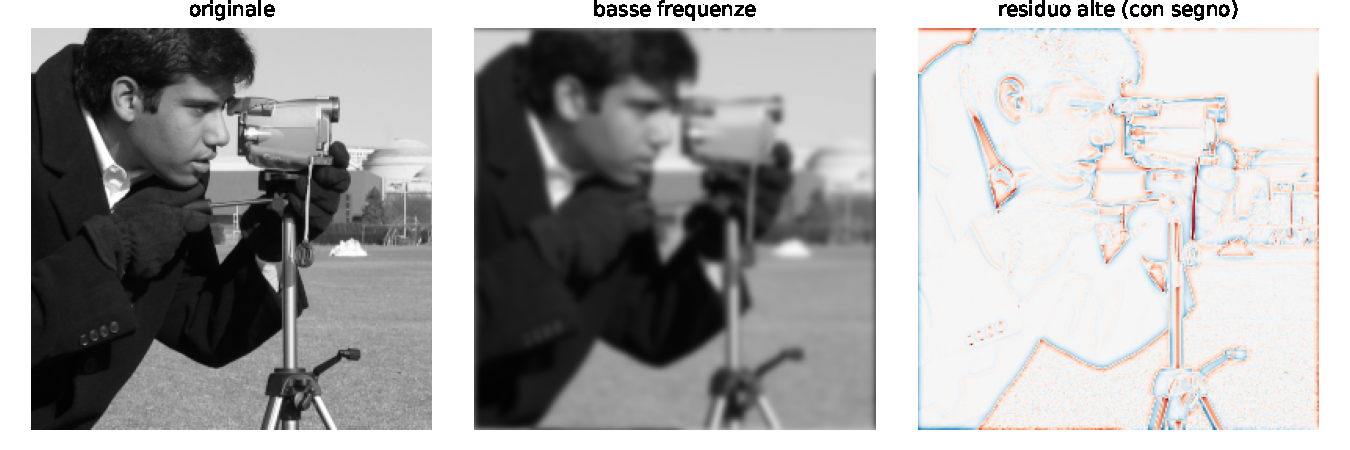
\includegraphics[width=0.85\linewidth]{fig/highpass.pdf}
\caption{Il residuo alto contiene bordi, tessiture fini e rumore insieme: un passa-basso non può togliere il rumore senza togliere anche i dettagli.}
\end{figure}

\subsection{Togliere un'interferenza periodica (filtro notch)}

Se il disturbo è un'onda a frequenza nota, nello spettro è \textbf{una coppia di picchi}. Si azzerano solo quelli, con una maschera \emph{notch} (``tacca''): 1 ovunque tranne due piccole gaussiane rovesciate sui due picchi coniugati.
\begin{Verbatim}
mask *= 1 - np.exp(-d2 / (2*width**2))   # per ognuno dei due picchi, width = 1/W
\end{Verbatim}

\begin{figure}[H]\centering
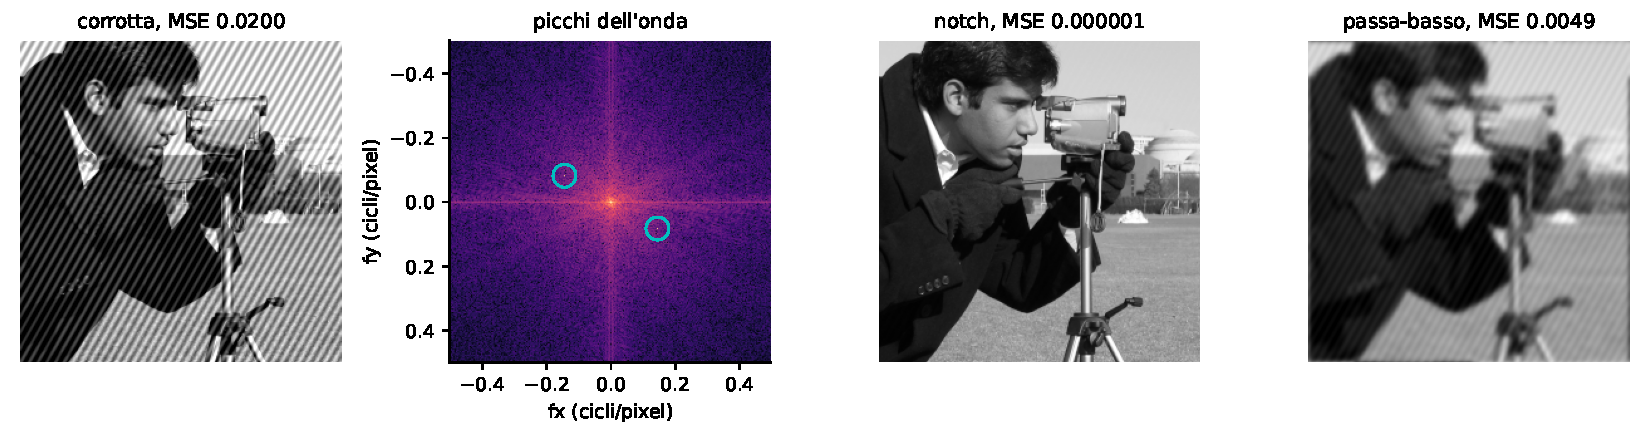
\includegraphics[width=\linewidth]{fig/notch_demo.pdf}
\caption{Onda di ampiezza 0.20 a $(k_x, k_y) = (37, 21)$ sommata a \code{camera}.}
\end{figure}

\begin{center}
\begin{tabular}{@{}lc@{}}
\toprule
Immagine & MSE rispetto all'originale (rieseguito = salvato) \\
\midrule
Corrotta & 0.020000 \\
Notch & 0.000001 \\
Passa-basso gaussiano & 0.004886 \\
\bottomrule
\end{tabular}
\end{center}
0.02 non è un caso: la media di $(A\cos)^2$ è $A^2/2 = 0.2^2/2 = 0.02$. Il notch toglie quasi solo il disturbo; il passa-basso toglie il disturbo ma sfoca l'immagine.

\subsection{Esercizio 1: la foto corrotta (\code{corrupted\_photo.npy})}

\begin{soluzione}
\begin{enumerate}
  \item \textbf{Trovare i picchi}: si calcola \code{abs(fft2(obs))}, si ignora il centro ($r < 0.05$, dove c'è l'immagine) e si prende il massimo. Risultato: una sola coppia, $(k_y, k_x) = \pm(-43, 29)$, circa 400 volte sopra i vicini. Ampiezza dell'onda $2|F|/(HW) = 0.181$.
  \item \textbf{Maschera}: \code{notch\_mask(obs.shape, 29/256, -43/256, width=1/256)}, la stessa funzione del notebook.
  \item \textbf{Ricostruire}: \code{ifft2(Fo * notch).real}.
  \item \textbf{Confronto}: l'immagine pulita è \code{data.coffee()} di scikit-image, in grigio e ridotta a $256 \times 256$ (trovata confrontando con le immagini di esempio della libreria). Rispetto a quella: osservata MSE 0.0162, notch $1.8 \cdot 10^{-6}$, gaussiano ($\sigma = 2$) 0.0034.
\end{enumerate}
\end{soluzione}

\begin{figure}[H]\centering
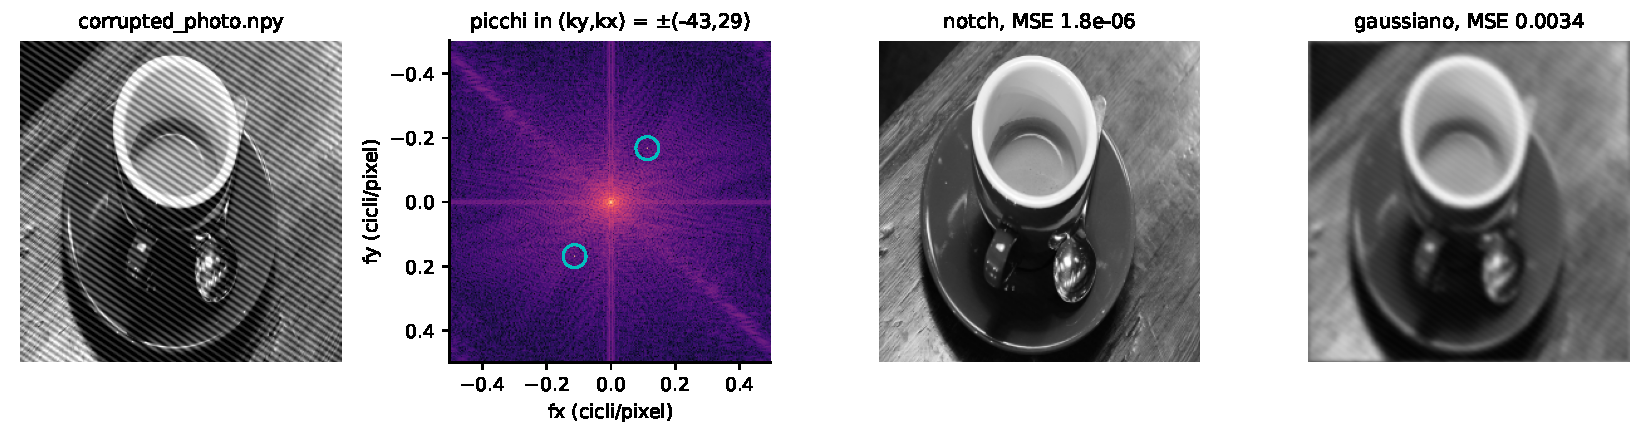
\includegraphics[width=\linewidth]{fig/notch_exercise.pdf}
\end{figure}

\subsection{Esercizio 2: compressione con Fourier (Fig.~16.8 del visionbook)}

\begin{soluzione}
Si tengono solo i coefficienti di modulo più grande e si azzerano gli altri:
\begin{Verbatim}
thr = np.sort(np.abs(F).ravel())[::-1][int(keep*F.size) - 1]
rec = np.fft.ifft2(np.where(np.abs(F) >= thr, F, 0)).real
\end{Verbatim}
I due coefficienti coniugati hanno lo stesso modulo, quindi vengono tenuti o buttati insieme e la ricostruzione resta reale.

\begin{center}
\begin{tabular}{@{}lccc@{}}
\toprule
Coefficienti tenuti & quanti & MSE & PSNR \\
\midrule
20\% & 13107 & 0.00068 & 31.7 dB \\
5\% & 3276 & 0.00267 & 25.8 dB \\
1\% & 655 & 0.00776 & 21.1 dB \\
0.2\% & 131 & 0.01674 & 17.8 dB \\
\bottomrule
\end{tabular}
\end{center}
\end{soluzione}

\begin{figure}[H]\centering
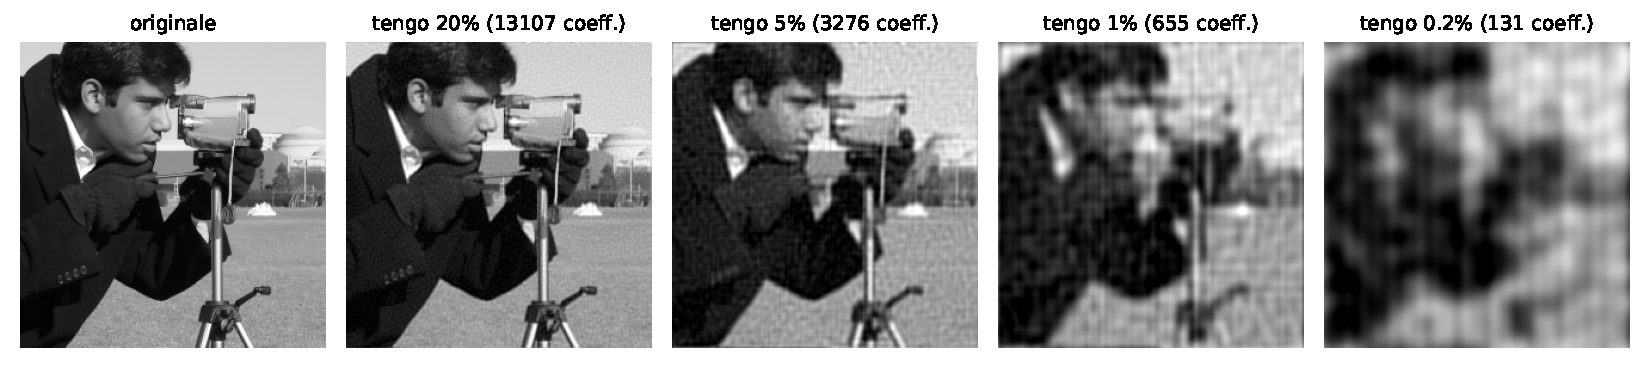
\includegraphics[width=\linewidth]{fig/compression.pdf}
\caption{Con il 5\% dei coefficienti l'immagine è ancora riconoscibile: l'energia è concentrata in pochi coefficienti a bassa frequenza. Scendendo, compaiono sfocatura e ringing.}
\end{figure}

\begin{attenzione}
\textbf{1. Figura vuota.} La cella 2 chiama \code{plt.figure()} prima di \code{plt.matshow(FY)}: \code{matshow} crea già la sua figura, quindi resta una figura vuota (nell'output salvato: \code{<Figure size 704x528 with 0 Axes>}).

\textbf{2. ``Shift'' vuol dire shift circolare.} La proprietà ``lo spostamento cambia solo la fase'' vale esatta per \code{np.roll}. Per uno spostamento vero (con pixel nuovi che entrano dal bordo) il modulo cambia un po'.

\textbf{3. Numeri diversi di poco.} Errore di ricostruzione salvato $6.66 \cdot 10^{-16}$, rieseguito $5.55 \cdot 10^{-16}$: dipende dalla versione di NumPy, non è un errore.
\end{attenzione}

\begin{esame}
\begin{itemize}[leftmargin=*]
  \item Onda $\Rightarrow$ coppia di picchi coniugati, perpendicolari alle strisce. Frequenza non intera $\Rightarrow$ leakage.
  \item Traslazione = rampa di fase; il modulo non cambia.
  \item Filtrare con la FFT = convoluzione circolare (\code{wrap}).
  \item Passa-basso ideale $\Rightarrow$ ringing (overshoot del 9\%); gaussiano no.
  \item Interferenza periodica: notch sui due picchi, molto meglio di un passa-basso (MSE $10^{-6}$ contro $5 \cdot 10^{-3}$).
\end{itemize}
\end{esame}

\newpage
%=====================================================================
\section{Classificare con banchi di filtri fissi (\code{filter\_bank.ipynb})}

\begin{idea}
Invece di imparare i filtri (come una CNN), li si sceglie a mano: si convolve l'immagine con ogni filtro, si applica una non linearità, si riduce con il pooling e si dà tutto a un classificatore \emph{lineare}. Il laboratorio misura quanto conta ogni scelta: quali filtri, quale non linearità, quanto pooling.
\end{idea}

\subsection{Pipeline e dati}

\[
x \;\longrightarrow\; x * w_k \;\longrightarrow\; \rho(x * w_k) \;\longrightarrow\; P\big(\rho(x * w_k)\big) \;\longrightarrow\; \text{classificatore lineare}
\]

\begin{center}
\begin{tabular}{@{}lp{10.5cm}@{}}
\toprule
Passo & Nel codice \\
\midrule
Convoluzione & \code{signal.fftconvolve(..., mode="same")}, zero padding \\
Non linearità $\rho$ & \code{none}, \code{abs} $|r|$, \code{square} $r^2$, \code{rectify} $\max(r,0)$ \\
Pooling $P$ & blocchi $p \times p$ non sovrapposti, media (\code{avg}) o massimo (\code{max}) \\
\code{power} & $z \leftarrow \text{sign}(z)|z|^{\text{power}}$, opzionale \\
Classificatore & \code{StandardScaler} + \code{RidgeClassifier(alpha=1)}, fisso \\
\bottomrule
\end{tabular}
\end{center}

\begin{itemize}
  \item \textbf{Dati}: Fashion-MNIST, immagini $28 \times 28$ di vestiti in 10 classi. Train 20000, validazione 10000 (dal training set ufficiale, senza sovrapposizione), test 10000. Il notebook li scarica da solo in \code{lab/data} (30 MB, già scaricati).
  \item \textbf{Numero di feature} = filtri $\times (28/p)^2$. Con pool 4: 49 per filtro.
  \item Si confrontano le scelte sulla \textbf{validazione}; il test si usa solo alla fine.
\end{itemize}

\begin{idea}
\textbf{Perché serve la non linearità.} Convoluzione e pooling medio sono lineari: senza $\rho$ le feature sono combinazioni lineari dei pixel, e un classificatore lineare su di esse non può fare meglio che sui pixel. Verificato: 7 filtri, \code{none}, pool 1 (5488 feature) $\to$ 0.8127, pixel grezzi 0.8129.
\end{idea}

\subsection{Come leggere i numeri}

Le soluzioni degli esercizi sono state tolte dal notebook (\code{assert False}), ma sono rimasti gli output del docente. Ho ricostruito le soluzioni e rieseguito tutto. Per tarare il confronto: le celle con codice completo (Gabor) danno valori diversi al massimo di 0.0004 da quelli salvati, per le versioni diverse delle librerie. Differenze più grandi indicano che il docente ha usato un filtro un po' diverso.

\begin{figure}[H]\centering
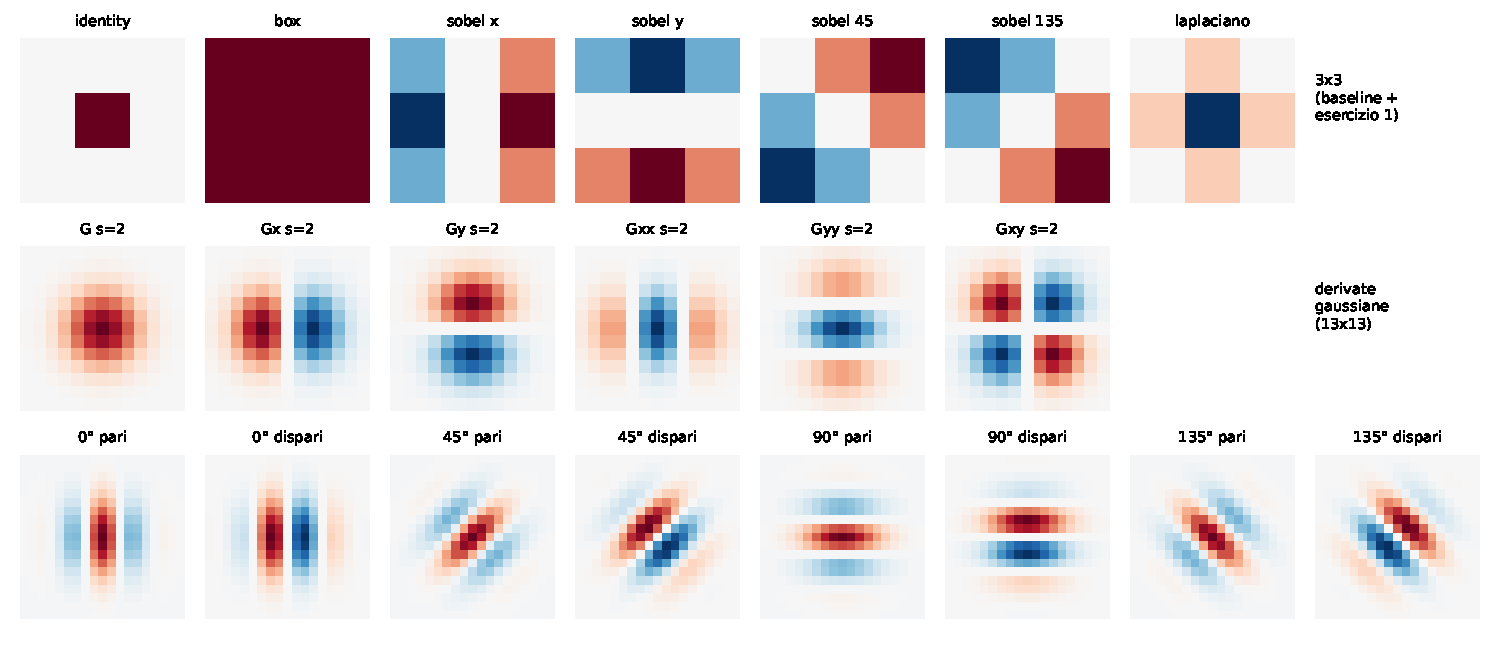
\includegraphics[width=\linewidth]{fig/banks.pdf}
\caption{I filtri usati. Rosso positivo, blu negativo. Riga 3: Gabor a $\sigma = 3$, $\lambda = 8$, 4 orientazioni, fase pari (coseno) e dispari (seno).}
\end{figure}

\subsection{Pixel e baseline (identity, box, Sobel)}

\begin{soluzione}
\begin{Verbatim}
box     = np.ones((3, 3)) / 9
sobel_x = np.array([[-1, 0, 1], [-2, 0, 2], [-1, 0, 1]], float)
sobel_y = sobel_x.T
\end{Verbatim}
\end{soluzione}

\begin{center}
\begin{tabular}{@{}lccc@{}}
\toprule
Configurazione & feature & salvato & rieseguito \\
\midrule
Pixel grezzi (identity, \code{none}, pool 1) & 784 & 0.8128 & 0.8129 \\
Baseline (identity, box, Sobel x/y; \code{abs}, pool 4) & 196 & 0.8376 & 0.8381 \\
Baseline senza identity & 147 & & 0.8343 \\
Solo identity, \code{abs}, pool 4 & 49 & & 0.7498 \\
\bottomrule
\end{tabular}
\end{center}

\textbf{QB.1} Con identity 0.8381, senza 0.8343: il pixel grezzo aiuta poco. La baseline batte i pixel con 4 volte meno feature: il pooling riassume ogni blocco $4 \times 4$ ed è tollerante a piccoli spostamenti; da solo però perde troppo (identity + pool 4: 0.7498). Servono i filtri di bordo prima del pooling.

\textbf{QB.2} (risposta nel notebook) Sobel x risponde ai bordi verticali: pantaloni, vestiti, borse. Sobel y ai bordi orizzontali: cinghie dei sandali, orli e maniche. Il rapporto tra le due risposte in ogni blocco è un descrittore grezzo dell'orientazione.

\begin{figure}[H]\centering
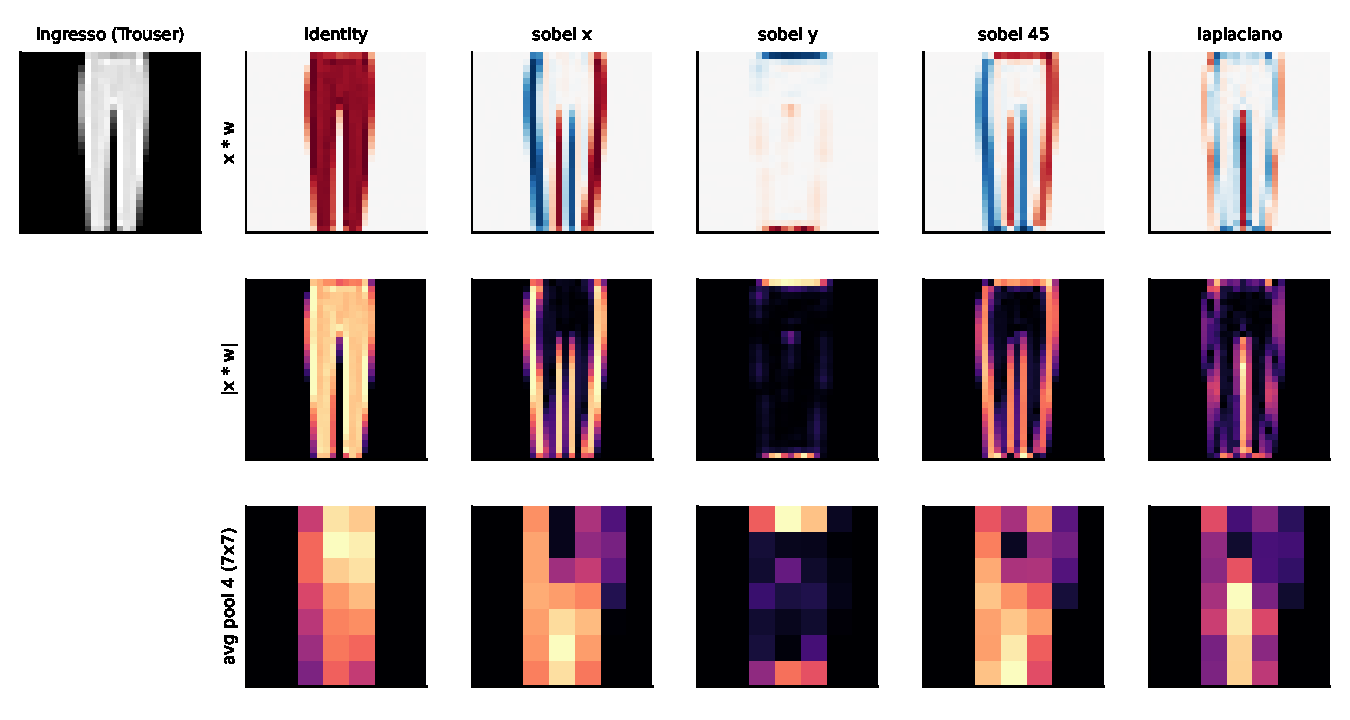
\includegraphics[width=0.85\linewidth]{fig/responses.pdf}
\caption{Un pantalone attraverso la pipeline. Sobel x vede le gambe, Sobel y quasi niente. L'ultima riga (7 $\times$ 7 = 49 numeri per filtro) è quello che vede il classificatore.}
\end{figure}

\subsection{Esercizio: diagonali e laplaciano}

\begin{soluzione}
\begin{Verbatim}
sobel_d45  = np.array([[0, 1, 2], [-1, 0, 1], [-2, -1, 0]], float)
sobel_d135 = np.array([[-2, -1, 0], [-1, 0, 1], [0, 1, 2]], float)
laplacian  = np.array([[0, 1, 0], [1, -4, 1], [0, 1, 0]], float)   # 4-vicini
\end{Verbatim}
Stessa idea di Sobel: derivata attraverso il bordo, media lungo il bordo, ruotata di 45 gradi.
\end{soluzione}

\begin{center}
\begin{tabular}{@{}lccc@{}}
\toprule
Banco & feature & salvato & rieseguito \\
\midrule
baseline + diagonali & 294 & 0.8573 & 0.8600 \\
baseline + laplaciano & 245 & 0.8456 & 0.8484 (4-vicini) / 0.8460 (8-vicini) \\
baseline + diagonali + laplaciano & 343 & 0.8638 & 0.8641 \\
\bottomrule
\end{tabular}
\end{center}

\textbf{Risposta}: le diagonali aiutano di più (+2.2 punti contro +1.0 del laplaciano): aggiungono orientazioni che Sobel x/y non coprono. Il laplaciano è isotropo, quindi non aggiunge informazione di orientazione.

\subsection{Esercizio: derivate gaussiane a più scale}

\begin{soluzione}
Per ogni $\sigma$: la gaussiana e le 5 derivate già implementate (\code{x}, \code{y}, \code{xx}, \code{yy}, \code{xy}), più una identity in testa. Con una scala sono 7 filtri = 343 feature, lo stesso numero dell'output salvato.
\begin{Verbatim}
gd_bank = [identity] + [k for s in sigmas for k in
           [gaussian_kernel(s)] + [gaussian_derivative_kernel(s, o)
                                   for o in ["x", "y", "xx", "yy", "xy"]]]
\end{Verbatim}
\end{soluzione}

\begin{center}
\begin{tabular}{@{}lccc@{}}
\toprule
Scale $\sigma$ & feature & salvato & rieseguito \\
\midrule
1 & 343 & 0.8583 & 0.8634 \\
2 & 343 & 0.8562 & 0.8605 \\
1, 2 & 637 & 0.8748 & 0.8809 \\
0.7, 1, 2, 3 & 1225 & 0.8865 & 0.8905 \\
\bottomrule
\end{tabular}
\end{center}

Una scala sola vale come i 7 filtri $3 \times 3$; \textbf{più scale insieme} aiutano (+2.7 punti rispetto a $\sigma = 1$), perché vedono sia i dettagli fini sia le strutture larghe (spazio tra le gambe, colletto). Ipotesi sulla differenza di circa 0.5 punti dai valori salvati: il docente ha usato un banco di 7 filtri un po' diverso (non ricostruibile dagli output).

\subsection{Filtri di Gabor}

Un filtro di Gabor è una gaussiana moltiplicata per un'onda: risponde a una \emph{posizione}, una \emph{orientazione} $\theta$ e una \emph{frequenza} $1/\lambda$. Somigliano alle cellule semplici della corteccia visiva (V1) e ai filtri del primo strato delle CNN. Codice già completo nel notebook.

\begin{center}
\begin{tabular}{@{}lccc@{}}
\toprule
Orientazioni (x 2 scale x 2 fasi, + identity) & feature & salvato & rieseguito \\
\midrule
2 & 441 & 0.8673 & 0.8675 \\
4 & 833 & 0.8865 & 0.8867 \\
8 & 1617 & 0.8949 & 0.8945 \\
\bottomrule
\end{tabular}
\end{center}

Più orientazioni = più accuratezza, con guadagno che cala (2$\to$4: +1.9 punti, 4$\to$8: +0.8).

\subsection{Esercizio: non linearità e pooling}

\begin{figure}[H]\centering
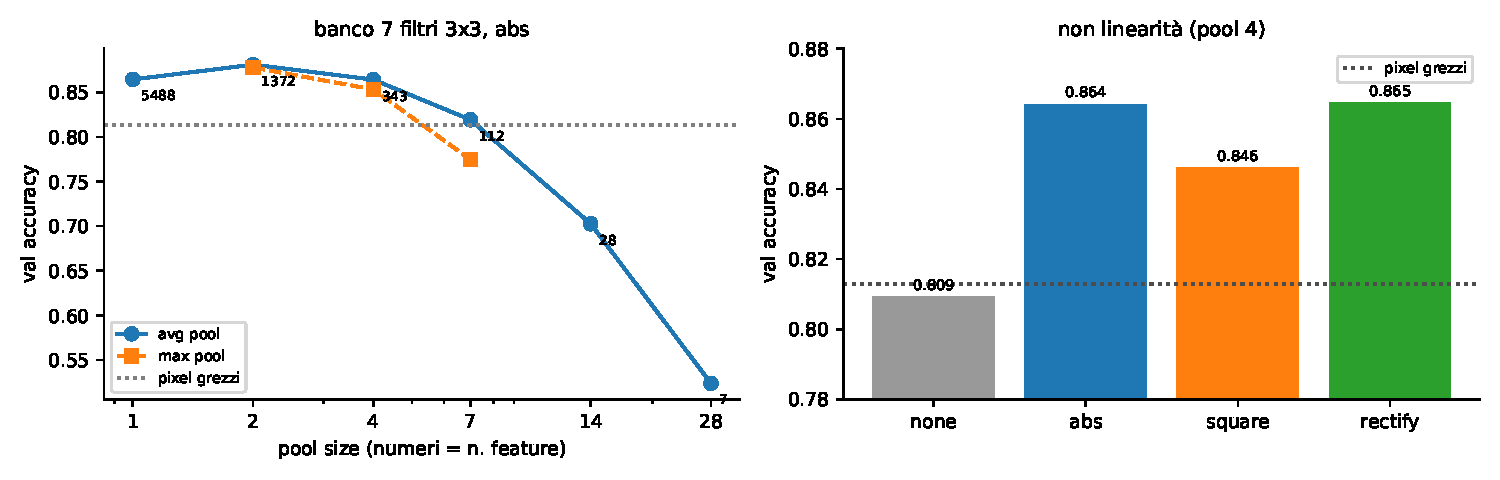
\includegraphics[width=\linewidth]{fig/pooling.pdf}
\caption{Banco a 7 filtri $3 \times 3$ (baseline + diagonali + laplaciano), rieseguito.}
\end{figure}

\begin{center}
\begin{tabular}{@{}lcc|lcc@{}}
\toprule
Non linearità (pool 4) & val & & Pooling (\code{abs}, media) & feature & val \\
\midrule
\code{none} & 0.8092 & & 1 & 5488 & 0.8644 \\
\code{abs} & 0.8641 & & 2 & 1372 & \textbf{0.8809} \\
\code{square} & 0.8461 & & 4 & 343 & 0.8641 \\
\code{rectify} & \textbf{0.8646} & & 7 & 112 & 0.8192 \\
\code{abs} + \code{power=0.5} & 0.8715 & & 14 / 28 & 28 / 7 & 0.7026 / 0.5238 \\
\bottomrule
\end{tabular}
\end{center}

Max pooling (\code{abs}): 0.8777 (pool 2), 0.8531 (pool 4), 0.7746 (pool 7), sempre sotto la media.

Risposte alle domande:
\begin{itemize}
  \item \textbf{Senza non linearità}: verificato, non si supera il pixel grezzo (0.8127 con pool 1, 0.8092 con pool 4, contro 0.8129).
  \item \textbf{Pooling}: si guadagna tolleranza ai piccoli spostamenti e meno feature (meno rischio di overfitting, più veloce); si perde la posizione. Il migliore qui è pool 2; oltre 4 si perde troppo (pool 28 = un numero per filtro: 0.52).
  \item \textbf{\code{power=0.5}} (+0.7 punti): comprime i valori grandi, così poche risposte fortissime non dominano il classificatore lineare. Spiegazione standard, non misurata qui.
  \item \code{square} va peggio di \code{abs}: eleva al quadrato proprio i valori grandi, l'effetto opposto di \code{power=0.5}.
\end{itemize}

\subsection{Esercizio: filtri casuali}

\begin{soluzione}
\begin{Verbatim}
rng = np.random.default_rng(0)
def random_bank(n, size=5):
    return [rng.standard_normal((size, size)) for _ in range(n)]
\end{Verbatim}
\end{soluzione}

\begin{center}
\begin{tabular}{@{}lcccc@{}}
\toprule
Filtri casuali $5 \times 5$ & feature & salvato & rieseguito (seed 0) & banco a mano con stesse feature \\
\midrule
4 & 196 & 0.8349 & 0.8361 & baseline 0.8381 \\
13 & 637 & 0.8714 & 0.8774 & derivate gauss. $\sigma = 1,2$: 0.8809 \\
34 & 1666 & 0.8922 & 0.8925 & Gabor 8: 0.8945 \\
\bottomrule
\end{tabular}
\end{center}

\textbf{Q6.1}: con abbastanza filtri, i casuali arrivano quasi ai banchi fatti a mano. \textbf{Q6.2}: i casuali non richiedono progettazione ma non si sa cosa misurano (poco interpretabili) e servono più filtri per lo stesso risultato; quelli a mano sono interpretabili (``bordo a 45 gradi'') e più efficienti a parità di feature.

\subsection{Challenge e test finale}

Output salvati del docente (composizione esatta dei banchi non nota, quindi non rieseguiti):
\begin{center}
\begin{tabular}{@{}lcc@{}}
\toprule
Configurazione del docente & feature & val \\
\midrule
energia di Gabor 8x2 (``complex cells''), power 0.5 & 882 & 0.8884 \\
Gabor 8, power 0.5 & 1666 & 0.9002 \\
Gabor 8x3 + derivate gaussiane, power 0.5 & 3038 & 0.9094 \\
\bottomrule
\end{tabular}
\end{center}
L'\emph{energia di Gabor} è $\sqrt{r_{\text{pari}}^2 + r_{\text{dispari}}^2}$: la risposta non dipende dalla fase, come nelle cellule complesse di V1.

Test (riallenando su train + validazione), rieseguito:
\begin{center}
\begin{tabular}{@{}lc@{}}
\toprule
Configurazione & test accuracy \\
\midrule
Pixel grezzi & 0.8101 \\
Baseline & 0.8383 \\
Baseline, power 0.5 & 0.8557 \\
Gabor 8 + identity, power 0.5 (val 0.9055) & \textbf{0.8983} \\
\bottomrule
\end{tabular}
\end{center}

\begin{attenzione}
{\small Numeri di cella = numerazione del notebook originale.}

\textbf{1. \code{'ReLU'} non esiste.} Il testo (cella 5) chiama la non linearità \code{'ReLU'}, ma nel dizionario \code{NONLINEARITIES} la chiave è \code{'rectify'}: \code{nonlinearity="ReLU"} dà \code{KeyError}.

\textbf{2. Il banco finale non è il migliore.} Cella 32: \code{FINAL\_BANK = baseline\_bank \# best validation entry}. Il commento chiede di mettere il banco migliore, il codice mette la baseline. Va sostituito con il proprio banco migliore.

\textbf{3. Output da esecuzioni diverse.} La cella 32 ha salvato un \code{NameError} (\code{baseline\_bank} non definito), ma la cella 34, che usa le stesse variabili, ha un grafico: gli output salvati non vengono da un'unica esecuzione dall'alto in basso.

\textbf{4. \code{show\_responses} usa sempre pool 4.} Disegna \code{pool(..., 4).reshape(7, 7)} qualunque sia il \code{pool\_size} provato: le mappe mostrate non cambiano se si cambia il pooling.
\end{attenzione}

\begin{esame}
\begin{itemize}[leftmargin=*]
  \item Filtri lineari + classificatore lineare = classificatore lineare sui pixel. Serve una non linearità ($|\cdot|$, ReLU).
  \item Pooling: tolleranza a piccoli spostamenti e meno feature, al prezzo della posizione. C'è un punto ottimo (qui pool 2).
  \item Più orientazioni e più scale aiutano. Filtri casuali in numero sufficiente arrivano vicino a quelli a mano.
  \item Manca la gerarchia (filtri su filtri) e l'apprendimento dei filtri: è quello che aggiunge una CNN.
\end{itemize}
\end{esame}

%=====================================================================
\section{Image blending (\code{06-image-blending})}

Il notebook in \code{lab/06-image-blending} è \textbf{identico byte per byte} a quello della lezione 6 (stesso hash MD5). È già spiegato in \code{Appunti/CV\_L6\_Aliasing\_Scale\_Invariance\_appunti.txt}, parte B, con i due bug verificati e la figura \code{L6\_blending\_confronto.png}.

In breve: piramide laplaciana di mela e arancia, piramide gaussiana della maschera, somma pesata livello per livello, ricostruzione (multi-band blending, Burt e Adelson 1983). Le bande basse si mescolano su una zona larga, quelle alte su una stretta: niente cucitura visibile e niente effetto ``fantasma''.

\bigskip
%=====================================================================
\section{Domande tipo esame}

\begin{enumerate}[leftmargin=*,itemsep=6pt]
  \item \textbf{Dove sono i picchi dello spettro di $\cos(2\pi(k_x x/W + k_y y/H))$?}\\
  In $\pm(k_y, k_x)$, di modulo $HW/2$. La direzione è perpendicolare alle strisce.
  \item \textbf{Cosa succede allo spettro se sposto l'immagine?}\\
  Il modulo resta uguale, la fase si moltiplica per $e^{-2\pi i(f_y d_y + f_x d_x)}$ (spostamento circolare).
  \item \textbf{Perché il passa-basso ideale dà aloni e il gaussiano no?}\\
  Il taglio netto corrisponde a una sinc nello spazio, che oscilla (overshoot del 9\% su un bordo). La gaussiana resta gaussiana, positiva, senza oscillazioni.
  \item \textbf{Come si toglie un disturbo periodico?}\\
  Si trovano i due picchi coniugati nello spettro e si azzerano con un filtro notch. Molto meglio di un passa-basso, che sfoca tutto.
  \item \textbf{Che condizione al bordo usa il filtraggio con la FFT?}\\
  Periodica (\code{wrap}): la DFT tratta l'immagine come ripetuta.
  \item \textbf{Perché in un banco di filtri serve la non linearità?}\\
  Senza, le feature sono lineari nei pixel e il classificatore lineare non migliora (0.8127 contro 0.8129).
  \item \textbf{Vantaggi e svantaggi del pooling?}\\
  Tolleranza a piccoli spostamenti, meno feature; si perde la posizione. Troppo pooling fa crollare l'accuratezza.
  \item \textbf{Cosa manca a un banco di filtri fissi rispetto a una CNN?}\\
  Filtri imparati dai dati e più strati (gerarchia).
\end{enumerate}

\section*{Cosa è verificato e cosa no}
\begin{itemize}
  \item \textbf{Rieseguito} con il codice dei notebook: tutte le celle di \code{demo.ipynb} (numeri stampati coincidenti con gli output salvati), le due soluzioni degli esercizi, il comportamento di \code{boundary="symm"}, la deviazione standard del kernel della maschera gaussiana. Tutti gli esperimenti di \code{filter\_bank.ipynb} nelle tabelle con colonna ``rieseguito'', compreso il test finale. Script e risultati in \code{Lessons/L7/appunti\_src/} (\code{verifica\_demo.py}, \code{verifica\_filter\_bank.py}, \code{risultati\_filter\_bank.json}, \code{figs.py}).
  \item \textbf{Non rieseguito}: la tabella della challenge (output salvati del docente). Le soluzioni degli esercizi di \code{filter\_bank} sono ricostruite da me: coincidono con gli output salvati per numero di feature, e per accuratezza entro 0.6 punti.
  \item \textbf{Ambiente}: numpy 2.5.3, scipy 1.18.1, scikit-image 0.26.0, scikit-learn 1.9.1, matplotlib 3.11.2.
\end{itemize}

\end{document}
